\documentclass{article}

\usepackage[brazilian]{babel}
\usepackage[utf8]{inputenc}
\usepackage[T1]{fontenc}
\usepackage{amsmath}
\usepackage{MnSymbol}
\usepackage{wasysym}
\usepackage{mdframed}
\usepackage[a4paper, total={6in, 10.5in}]{geometry}
\usepackage{graphicx}
\usepackage{caption}
\graphicspath{ {baciasNewton/} }

\title{MAC0210 - Laboratório de Métodos Numéricos}
\author{Exercício-programa 2}
\date{ }


\begin{document}

\maketitle

\begin{center}
\large{Vítor Kei Taira Tamada - 8516250}

\large{André Ferrari Moukarzel - 9298166}
\end{center}

\bigskip
\textbf{\Large{Decisões de projeto}}

\quad A implementação dos métodos como dada no enunciado deixa um problema claro a ser resolvido: a interpolação nas bordas em ambos os métodos.

\bigskip
\textbf{\large{1) Interpolação bilinear}}

\quad Primeiramente, o valor de cada ponto da nova imagem é encontrado segundo a fórmula dada no enunciado:

\begin{center}
$p_{ij}(x, y) = a_{0} + a_{1}(x - x_{i}) + a_{2}(y - y_{j}) + a_{3}(x - x_{i})(y - y_{j})$
\end{center}

\quad Em seguida, a distância $h$ entre dois pontos de mesma linha ou de mesma coluna é dividida em $k+1$ partes. Uma vez que o valor de $x$ da fórmula acima é maior do que $x_{i}$, temos que $x = x_{i} + d * \alpha$, sendo $d = \frac{h}{k+1}$ e $\alpha$ um inteiro tal que $0 \leq \alpha \leq k + 1$. Portanto,

\begin{center}
$x - x_{i} = x_{i} + d * \alpha - x_{i} = d * \alpha$
\end{center}

\quad Analogamente para $y = y_{j} + d * \beta$, temos

\begin{center}
$y - y_{j} = y_{j} + d * \beta - y_{j} = d * \beta$
\end{center}

\quad Percebe-se, então, que $x_{i}$ e $y_{j}$ afetam o valor de $p_{ij}$ apenas indiretamente por meio de influência nos valores de $a_{0}$, $a_{1}$, $a_{2}$ e $a_{3}$.

\quad Os valores de $\alpha$ e $\beta$, por suas vezes, fazem com que não apenas as bordas do quadrante sejam percorridas, mas os cantos $(x_{i}, y_{j})$, $(x_{i}, y_{j+1})$, $(x_{i+1}, y_{j})$ e $(x_{i+1}, y_{j+1})$ também. Como consequência, quase todas as bordas são percorridas e calculadas duas vezes e quase todos os cantos (pontos da imagem original) são percorridos e calculados quatro vezes.

\bigskip
\textbf{\large{2) Interpolação bicúbica}}

\quad Visto que as derivadas a serem utilizadas para a interpolação nas bordas são diferentes das do resto da imagem, decidimos tratá-las separadamente. Cada parte da "moldura" (borda superior, borda inferior, borda esquerda, borda direita, canto superior esquerdo, canto superior direito, canto inferior esquerdo e canto inferior direito) foi tratado separadamente, tendo seu próprio trecho de código no arquivo \texttt{decompress.m}.


\quad Para as bordas laterais, substituímos as derivadas de $x$ que não poderiam ser feitas de forma convencional pelas apresentadas no enunciado, além de adaptar as derivadas de segunda ordem ($\frac{\partial^{2}f}{\partial x \partial y}$) pelo mesmo motivo. Para as bordas superior e inferior, são substituídas as derivadas de $y$ necessárias.

\quad O cálculo de $p_{ij}(x, y)$ foi feito como definido pelo enunciado e os valores de $(x - x_{i})$ e $(y - y_{j})$ utilizados da mesma forma como na descompressão bilinear.

\bigskip
\textbf{\Large{3) Experimentos}}

\quad A descompressão se beneficia, isto é, mantém-se mais próxima da imagem original quanto mais contraste tiver. Isto acaba por se refletir em alguma diferença entre imagens com e sem cor - tendo uma imagem colorida e uma equivalente em tons de cinza, a colorida mantém-se mais fiel à original após ser descomprimida. A diferença, porém, é desprezível.

\quad A compressão, por outro lado, não é afetada pela presença ou ausência de cor.

\quad As operações com imagens apresentam resultados de qualidade equivalente para imagens geradas a partir de funções que são de classe $C^{2}$ e de funções que não são e até para imagens reais.

\quad Em todas as comparações de imagens feitas, o erro não passou de 2\%:

\qquad $\bullet$ Mesma imagem descomprimida pelo método da bilinear com $h = 0.1$ e $h = 1$ teve erro de $1.1379 * 10^{-4}$;

\qquad $\bullet$ Mesma imagem descomprimida pelo método da bicúbica com $h = 0.1$ e $h = 50$ teve erro de $0.013393$;

\qquad $\bullet$ Mesma imagem descomprimida pelo método da bilinear com $h = 0.1$ e pelo método da bicúbica com $h = 0.1$ teve erro de $0.019312$.

\quad Conclui-se então que o valor de $h$ tem pouca influência na qualidade da imagem gerada.

\bigskip
\textbf{\Large{4) Testes}}

\quad Verificando o efeito de diferentes valores de $h$ para diferentes imagens, temos que

\qquad $\bullet$ descomprimindo uma imagem com $k = 10$:

\bigskip
%
\includegraphics[scale=.75]{quesha05.png}

\begin{center}

\includegraphics{quesha.png}

\emph{Original}

\bigskip

\includegraphics{quesha05.png}

\emph{$h = 0.5$}

\bigskip

\includegraphics{quesha50.png}

\emph{$h = 50$}
\end{center}

\newpage
\qquad $\bullet$ comprimindo uma imagem com $k = 7$ e descomprimindo:

\bigskip
\begin{center}

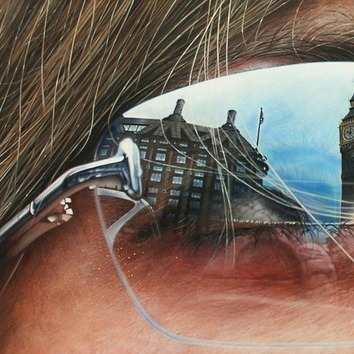
\includegraphics[scale=.8415]{real.png}

\emph{Original}

\bigskip

\includegraphics[scale=.63]{real1k_3vezes.png}

\emph{descomprimida com $k = 1$ três vezes}

\bigskip

\includegraphics[scale=.63]{real7k.png}

\emph{descomprimida com $k = 7$ uma vez}

\end{center}

\newpage
\qquad $\bullet$ imagem gerada pela função $f(x, y) = (sen(x), \frac{sen(y) + sen(x)}{2}, sen(x))$ e $k = 5$:

\begin{center}

\includegraphics{color.png}

\emph{Original}

\bigskip

\includegraphics[scale=.45]{bih01.png}

\emph{Descompressão bilinear com $h = 0.1$}

\emph{(imagem reduzida para caber no PDF)}

\bigskip

\includegraphics[scale=.45]{bih1.png}

\emph{Descompressão bilinear com $h = 1$}

\emph{(imagem reduzida para caber no PDF)}

\bigskip

\includegraphics[scale=.45]{cubi01.png}

\emph{Descompressão bicúbica com $h = 0.1$}

\emph{(imagem reduzida para caber no PDF)}

\bigskip

\includegraphics[scale=.45]{cubi50.png}

\emph{Descompressão bicúbica com $h = 50$}

\emph{(imagem reduzida para caber no PDF)}

\newpage
\qquad $\bullet$ imagem gerada pela função $f(x, y) = (sen(x), \frac{sen(y) + sen(x)}{2}, sen(x))$ em escalas de cinza:

\begin{center}

\includegraphics{gray.png}

\emph{Original}

\bigskip

\includegraphics{gray2.png}

\emph{$k = 2$ e $h - 0.5$}
\end{center}

\end{center}

\end{document}